\documentclass[10pt,twocolumn]{article}
% Tectonic compila con XeTeX (UTF-8 nativo): no usar inputenc/fontenc.
\usepackage[spanish,es-tabla]{babel}
\usepackage{graphicx}
\usepackage{booktabs}
\usepackage{amsmath}
\usepackage{url}
\usepackage[hidelinks]{hyperref}
\usepackage{geometry}
\geometry{letterpaper, margin=0.78in}
\setlength{\columnsep}{0.28in}

% Cifras generadas automaticamente por el pipeline (no editar a mano)
% Cifras clave generadas automaticamente — NO editar a mano.
\newcommand{\nJosse}{23{,}186}
\newcommand{\nJosseExp}{4,329}
\newcommand{\nSeera}{120}
\newcommand{\rdosJosseLin}{0.39}
\newcommand{\rdosSeeraRF}{0.81}
\newcommand{\rdosSeeraLin}{0.34}
\newcommand{\maeJosseLin}{0.49}
\newcommand{\maeJosseBase}{0.67}
\newcommand{\predQuinceJosse}{39.8\%}
\newcommand{\predTreintaJosse}{46.0\%}
\newcommand{\mdmreJosse}{33\%}
\newcommand{\rhoJosse}{0.79}
\newcommand{\predQuinceSeera}{16.7\%}
\newcommand{\subestSeera}{80.8\%}
\newcommand{\desvSeera}{58.6\%}
\newcommand{\mdmreSeera}{38\%}
\newcommand{\pCambio}{0.57}


\title{\Large\bfseries Estimación temprana de esfuerzo, tiempo y costo en proyectos de software para gobiernos municipales: propuesta metodológica para el control de cambios con referencia a Fresnillo, Zacatecas\\[4pt]
\large Análisis cuantitativo preliminar con los datasets públicos JOSSE y SEERA}
\author{Rogelio Flores Rodríguez\\
\small Ingeniería en Software, Universidad Autónoma de Zacatecas\\
\small Seminario de Investigación. Docente: Dra. Julieta Guadalupe Rodríguez Ruiz}
\date{\small Junio de 2026}

\begin{document}
\maketitle

\begin{abstract}
\noindent La estimación temprana de proyectos de software municipales se realiza con requerimientos incompletos, cambios frecuentes y poca evidencia histórica local, lo que favorece cotizaciones basadas en opinión y proyectos financieramente frágiles. Este trabajo aporta evidencia cuantitativa preliminar para una metodología de estimación integral, analizando dos datasets públicos de ingeniería de software: JOSSE (\nJosse{} tareas de desarrollo y mantenimiento con esfuerzo real registrado, de las cuales \nJosseExp{} cuentan con estimación experta) y SEERA (\nSeera{} proyectos desarrollados en entornos con restricciones técnicas y económicas). Los resultados muestran tres hechos relevantes para el contexto municipal. Primero, las estimaciones expertas correlacionan con el esfuerzo real ($\rho=\rhoJosse$) pero fallan en magnitud: solo \predQuinceJosse{} de las tareas anotadas cae dentro del umbral de precisión de $\pm$15\,\%. Segundo, en proyectos de entornos restringidos la subestimación es sistemática: \subestSeera{} de los proyectos de SEERA requirió más esfuerzo del estimado, con una desviación mediana de +\desvSeera. Tercero, variables disponibles en etapas tempranas permiten superar a la línea base: una regresión lineal sobre variables textuales alcanza $R^2=\rdosJosseLin$ en JOSSE y un bosque aleatorio sobre variables tempranas de proyecto alcanza $R^2=\rdosSeeraRF$ en SEERA. Estos hallazgos justifican el diseño de EMPS-Fresnillo, un prototipo que captura de forma estructurada requerimientos, modo de desarrollo, cambios, costos fiscales-laborales y flujo de efectivo para producir estimaciones auditables y, en una fase posterior, validarlas con casos locales.
\end{abstract}

\vspace{4pt}
\noindent\textbf{Palabras clave:} estimación temprana, esfuerzo de software, control de cambios, gobiernos municipales, datasets públicos, JOSSE, SEERA, Fresnillo.

\section{Introducción}
El software se ha convertido en infraestructura administrativa para los gobiernos municipales. Un sistema de trámites, recaudación, expedientes o atención ciudadana no es solamente una aplicación: modifica tiempos de respuesta, responsabilidades y evidencia documental. En el caso de Fresnillo, el Plan Municipal de Desarrollo 2025-2027 plantea fortalecer la gestión administrativa mediante procesos innovadores, eficientes y transparentes \cite{fresnillo2025}, lo que vuelve pertinente estudiar cómo se estiman y controlan los proyectos de software antes de que el costo, el calendario y el alcance se vuelvan difíciles de corregir.

En proyectos municipales la estimación temprana se realiza con información incompleta. Las áreas usuarias expresan necesidades en lenguaje general, sin distinguir si solicitan una pantalla, una regla de negocio, una integración o una obligación de auditoría. El proveedor, a su vez, suele cotizar con base en experiencia informal o presión comercial, sin calcular con precisión los cambios, el mantenimiento, las obligaciones fiscales y laborales mexicanas, ni el flujo de efectivo necesario para sostener el proyecto \cite{jorgensen2007}. El problema aumenta cuando el proyecto cambia: una solicitud aparentemente menor puede afectar arquitectura, datos, pruebas, capacitación y mantenimiento, y la literatura muestra que el costo de un cambio crece conforme avanza la fase del proyecto \cite{boehm1981}.

La pregunta que orienta este avance es: ¿en qué medida la evidencia disponible en datasets públicos de ingeniería de software respalda que (a) la estimación basada únicamente en juicio experto es insuficiente y (b) variables observables en etapas tempranas permiten construir estimaciones más útiles para proyectos municipales?

La hipótesis de trabajo del proyecto sostiene que una estimación temprana es más útil para un gobierno municipal y para un proveedor cuando no calcula únicamente horas de programación, sino la viabilidad completa del proyecto: claridad de requerimientos, modo de desarrollo, costo de cambios, obligaciones fiscales y laborales, flujo de efectivo y mantenimiento. Dado que aún no existe un historial local suficiente de proyectos municipales terminados en Fresnillo, este artículo aporta la fase cuantitativa preliminar de esa investigación con datos públicos, y deja la validación local como trabajo de la siguiente fase mediante el prototipo EMPS-Fresnillo.

Las contribuciones de este avance son tres: (1) un análisis reproducible de la precisión de estimaciones expertas sobre \nJosseExp{} tareas reales anotadas; (2) una cuantificación de la subestimación sistemática de esfuerzo en \nSeera{} proyectos de entornos restringidos, contexto comparable al de proveedores municipales mexicanos; y (3) una comparación de modelos de estimación construidos exclusivamente con variables tempranas, contra una línea base de promedio.

\section{Trabajos relacionados}
\subsection{Estimación temprana basada en artefactos textuales}
La investigación reciente sobre estimación temprana utiliza artefactos disponibles desde etapas iniciales, como historias de usuario, requerimientos e issues \cite{radlinski2025llm}. Esta orientación resulta adecuada para proyectos municipales, donde la información inicial proviene de solicitudes administrativas y descripciones generales. Los datasets públicos ofrecen una base para formular variables sin depender únicamente de intuición local: JOSSE permite contrastar tareas con esfuerzo real y estimaciones expertas \cite{alhamed2022josse}; SEERA reúne proyectos de organizaciones con restricciones técnicas y económicas \cite{mustafa2020seera}; y el Public Jira Dataset permite estudiar cambios y trazabilidad a gran escala \cite{montgomery2025publicjira}, aunque por su tamaño se reserva para una etapa posterior.

\subsection{Control de cambios y costo del cambio}
Los cambios de requerimientos deben tratarse como un proceso estructurado que incluye análisis de impacto, modificación, verificación y aceptación \cite{kong2025requirements}. Las historias de usuario facilitan el entendimiento compartido, pero se degradan si no se conservan las conversaciones y razones de negocio \cite{sporsem2025}. El análisis de impacto manual es costoso y propenso a omisiones, lo que ha motivado enfoques automatizados de identificación de requerimientos afectados \cite{etezadi2025}. Estas líneas respaldan la decisión de diseño central del prototipo: el costo de un cambio no debe capturarse como cifra manual, sino calcularse a partir de los artefactos afectados, la fase, la claridad y el modo de desarrollo.

\subsection{Herramientas generativas y productividad}
La evidencia sobre herramientas generativas no permite asumir un multiplicador universal de velocidad. Experimentos de campo con 4{,}867 desarrolladores reportaron un aumento promedio de 26\,\% en tareas completadas \cite{cui2025}, mientras que un ensayo aleatorizado con desarrolladores experimentados de código abierto encontró un aumento de 19\,\% en el tiempo de finalización al usar herramientas de inicios de 2025 \cite{becker2025}. Por ello, la metodología propuesta estima por fase (análisis, codificación, revisión, pruebas, documentación, despliegue, mantenimiento) en lugar de aplicar un descuento global por modo de desarrollo.

\section{Materiales y métodos}
\subsection{Diseño del estudio}
Se realizó un estudio cuantitativo exploratorio y reproducible sobre datasets públicos, como fase preliminar de una investigación de diseño de artefacto \cite{hevner2004}. El objetivo no fue producir un modelo de producción, sino verificar si la evidencia pública sostiene las premisas del modelo de estimación integral antes de la validación local.

\subsection{Datasets y preparación}
\textbf{JOSSE.} Se utilizó la base curada distribuida en SQLite (versión del 18 de septiembre de 2020), con \nJosse{} tareas de desarrollo y mantenimiento provenientes de 371 proyectos de código abierto (ecosistemas Apache, JBoss y Spring). Cada registro incluye el texto del issue (título y descripción), número de comentarios, número de actividades y el esfuerzo real registrado en los worklogs de Jira, convertido de segundos a horas. Un subconjunto de \nJosseExp{} tareas cuenta además con estimación experta de esfuerzo; los valores faltantes están codificados como $-1$ y fueron excluidos del análisis de precisión experta.

\textbf{SEERA.} Se utilizó el archivo ARFF principal con \nSeera{} proyectos de 42 organizaciones. Para el modelo predictivo se seleccionaron exclusivamente variables conocidas en etapas tempranas (duración estimada, tamaño estimado, esfuerzo estimado, puntos de objeto, tamaño de equipo, tipo de organización, dominio de aplicación, madurez contractual, entre otras; 21 en total), excluyendo de forma explícita variables post-hoc como duración real, costos incurridos y ganancia/pérdida del proyecto, para evitar fuga de información hacia los modelos.

\textbf{Variables derivadas.} Para JOSSE se construyeron variables tempranas a partir del texto: longitud en caracteres, número de palabras, proyecto de origen y una variable binaria que marca la presencia de términos asociados a cambio o mantenimiento (\textit{change, fix, bug, refactor, migrate, improve}, entre otros).

\subsection{Modelos y métricas}
Se compararon tres modelos: línea base por promedio, regresión lineal y bosque aleatorio (200 árboles). La regresión lineal se incluye por su explicabilidad; el bosque aleatorio como contraste no lineal. La variable objetivo se transformó con $\log(1+\text{esfuerzo})$ para reducir el efecto de valores extremos, práctica estándar en datos de esfuerzo con cola larga. La partición entrenamiento/prueba fue 75/25 con semilla fija. Las métricas fueron MAE, RMSE y $R^2$ sobre la escala logarítmica.

La precisión de las estimaciones humanas se evaluó con los indicadores clásicos de la literatura de estimación \cite{conte1986}: MRE (error relativo de magnitud), MMRE y MdMRE (media y mediana del MRE) y PRED($x$), definido como la proporción de estimaciones con MRE $\leq x$\,\%. Como referencia de precisión aceptable se adoptó el umbral de $\pm$15\,\% utilizado en prácticas de medición funcional \cite{ifpug2010}.

\subsection{Hipótesis operacionales}
\textbf{H1.} La estimación basada únicamente en juicio experto es insuficiente: se espera que una fracción mayoritaria de las estimaciones expertas (JOSSE) y de proyecto (SEERA) exceda el umbral de $\pm$15\,\%.
\textbf{H2.} Las tareas asociadas a cambio o mantenimiento presentan distribución de esfuerzo distinta a las demás; se contrasta con la prueba de Mann-Whitney sobre los dos grupos de JOSSE.
\textbf{H3.} Variables tempranas permiten superar a la línea base de promedio: se espera $R^2$ positivo y reducción de MAE en ambos datasets.

\section{Resultados}
\subsection{Precisión de las estimaciones expertas (H1)}
La Tabla~\ref{tab:expertos} resume la precisión de las \nJosseExp{} estimaciones expertas de JOSSE. La correlación de Spearman con el esfuerzo real es alta ($\rho=\rhoJosse$): los expertos ordenan bien las tareas de menor a mayor esfuerzo. Sin embargo, la magnitud falla: el error relativo mediano es \mdmreJosse{} y solo \predQuinceJosse{} de las estimaciones cae dentro del umbral de $\pm$15\,\%; incluso relajando el umbral a $\pm$30\,\% la cobertura llega apenas a \predTreintaJosse. La Figura~\ref{fig:expertos} muestra la dispersión alrededor de la diagonal de estimación perfecta.

\begin{table}[t]
\centering
\caption{Precisi\'on de las estimaciones expertas en JOSSE ($n=4329$ tareas anotadas).}
\label{tab:expertos}
\small
\begin{tabular}{lr}
\toprule
Indicador & Valor \\
\midrule
MMRE (error relativo medio) & 2.92 \\
MdMRE (error relativo mediano) & 0.33 \\
PRED(15) & 39.8\% \\
PRED(30) & 46.0\% \\
Tareas subestimadas & 24.0\% \\
Correlaci\'on de Spearman ($\rho$) & 0.79 \\
\bottomrule
\end{tabular}
\end{table}


En SEERA el patrón es más severo y directamente relevante para el contexto municipal (Tabla~\ref{tab:seera}): \subestSeera{} de los \nSeera{} proyectos requirió más esfuerzo del estimado, con una desviación mediana de +\desvSeera{} respecto a la estimación original, y solo \predQuinceSeera{} de los proyectos quedó dentro del umbral de $\pm$15\,\%. La Figura~\ref{fig:seera} ilustra que la gran mayoría de los puntos se ubica por encima de la diagonal: la subestimación no es excepcional sino sistemática.

\begin{table}[t]
\centering
\caption{Desviaci\'on entre esfuerzo estimado y real en SEERA ($n=120$ proyectos).}
\label{tab:seera}
\small
\begin{tabular}{lr}
\toprule
Indicador & Valor \\
\midrule
MMRE & 0.39 \\
MdMRE & 0.38 \\
PRED(15) & 16.7\% \\
PRED(30) & 30.8\% \\
Proyectos subestimados & 80.8\% \\
Desviaci\'on mediana del esfuerzo & +58.6\% \\
\bottomrule
\end{tabular}
\end{table}


\subsection{Modelos con variables tempranas (H3)}
La Tabla~\ref{tab:metricas} compara los tres modelos. En JOSSE, la regresión lineal sobre variables textuales tempranas reduce el MAE de \maeJosseBase{} (línea base) a \maeJosseLin{} y alcanza $R^2=\rdosJosseLin$; el bosque aleatorio obtiene un desempeño similar. En SEERA, el bosque aleatorio sobre las 21 variables tempranas de proyecto alcanza $R^2=\rdosSeeraRF$, frente a $R^2=\rdosSeeraLin$ de la regresión lineal y un valor negativo de la línea base. La Figura~\ref{fig:pred} muestra el ajuste de la regresión lineal en el conjunto de prueba de JOSSE; las Figuras~\ref{fig:distjosse} y \ref{fig:distseera} presentan las distribuciones de esfuerzo, con la asimetría de cola larga que motivó la transformación logarítmica.

\begin{table}[t]
\centering
\caption{M\'etricas de los modelos sobre $\log(1+\text{esfuerzo})$ (conjunto de prueba, partici\'on 75/25).}
\label{tab:metricas}
\scriptsize
\setlength{\tabcolsep}{3.5pt}
\begin{tabular}{llrrrrr}
\toprule
Dataset & Modelo & $n_{ent}$ & $n_{pru}$ & MAE & RMSE & $R^2$ \\
\midrule
JOSSE & L\'inea base & 17389 & 5797 & 0.667 & 0.870 & -0.000 \\
JOSSE & Reg.\ lineal & 17389 & 5797 & 0.486 & 0.680 & 0.389 \\
JOSSE & Bosque aleat. & 17389 & 5797 & 0.517 & 0.722 & 0.312 \\
SEERA & L\'inea base & 90 & 30 & 0.982 & 1.175 & -0.239 \\
SEERA & Reg.\ lineal & 90 & 30 & 0.660 & 0.856 & 0.342 \\
SEERA & Bosque aleat. & 90 & 30 & 0.363 & 0.462 & 0.808 \\
\bottomrule
\end{tabular}
\end{table}


\subsection{Tareas asociadas a cambio (H2)}
La Tabla~\ref{tab:dispersion} contrasta el esfuerzo de las tareas que contienen términos de cambio o mantenimiento en su texto (26\,\% del corpus) contra el resto. Las distribuciones no difieren de forma estadísticamente significativa (Mann-Whitney, $p=\pCambio$) y las medidas de dispersión son comparables. La Figura~\ref{fig:boxplot} confirma visualmente la similitud. Este resultado nulo es informativo: la sola presencia de palabras clave en el texto de una tarea no discrimina su esfuerzo, lo que indica que la detección léxica es una aproximación insuficiente para gestionar cambios.

\begin{table}[t]
\centering
\caption{Esfuerzo real (horas) seg\'un presencia de t\'erminos de cambio/mantenimiento en JOSSE. Mann-Whitney $p=0.57$.}
\label{tab:dispersion}
\scriptsize
\setlength{\tabcolsep}{3.5pt}
\begin{tabular}{lrrrrr}
\toprule
Grupo & $n$ & Mediana & Media & D.E. & RIC \\
\midrule
Con t\'erm.\ cambio & 6004 & 1.00 & 4.37 & 16.98 & 2.50 \\
Sin t\'erm.\ cambio & 17182 & 1.00 & 4.50 & 19.90 & 2.67 \\
\bottomrule
\end{tabular}
\end{table}


\begin{figure}[t]
\centering
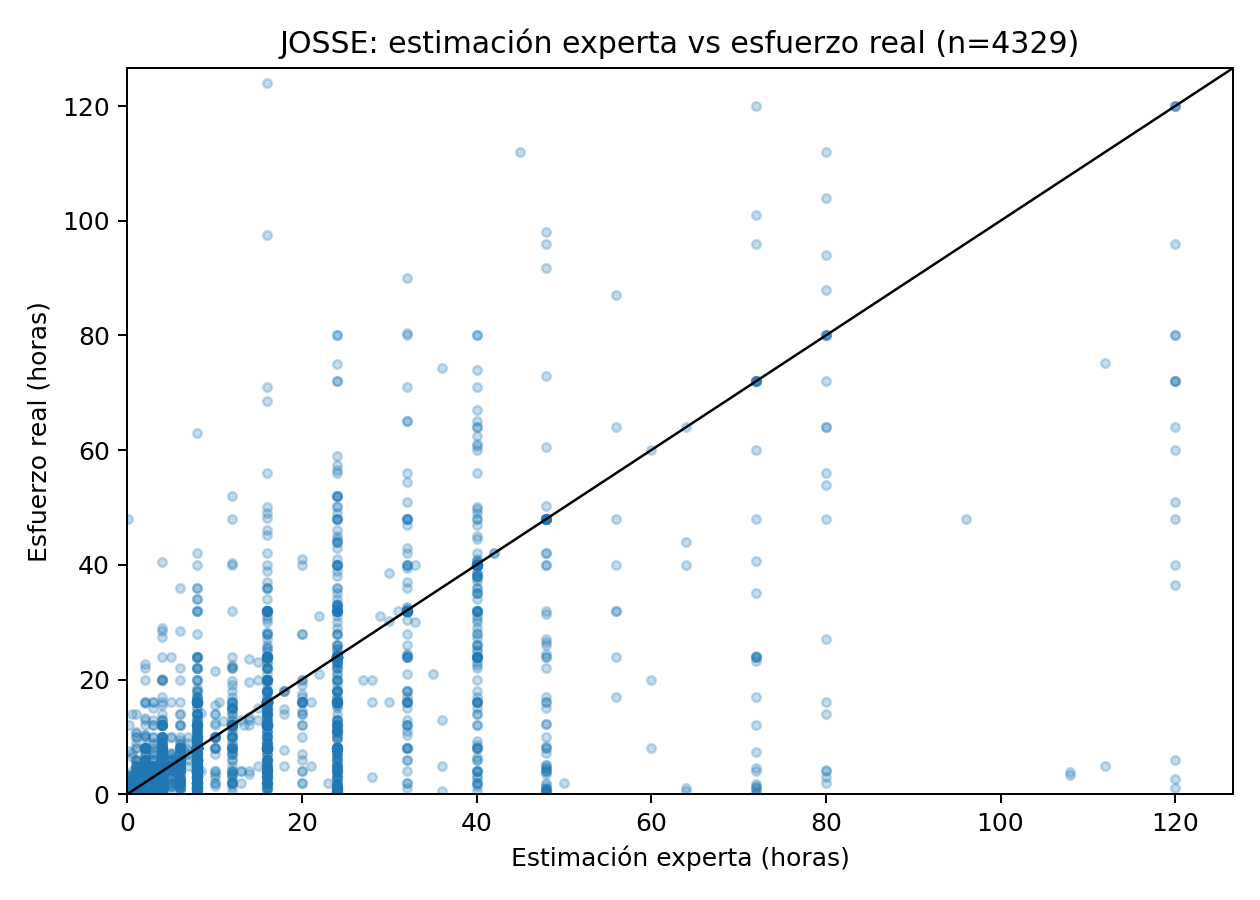
\includegraphics[width=0.95\linewidth]{../outputs/figures/josse_expert_vs_actual.png}
\caption{Estimaci\'on experta contra esfuerzo real en JOSSE. La l\'inea diagonal indica estimaci\'on perfecta.}
\label{fig:expertos}
\end{figure}

\begin{figure}[t]
\centering
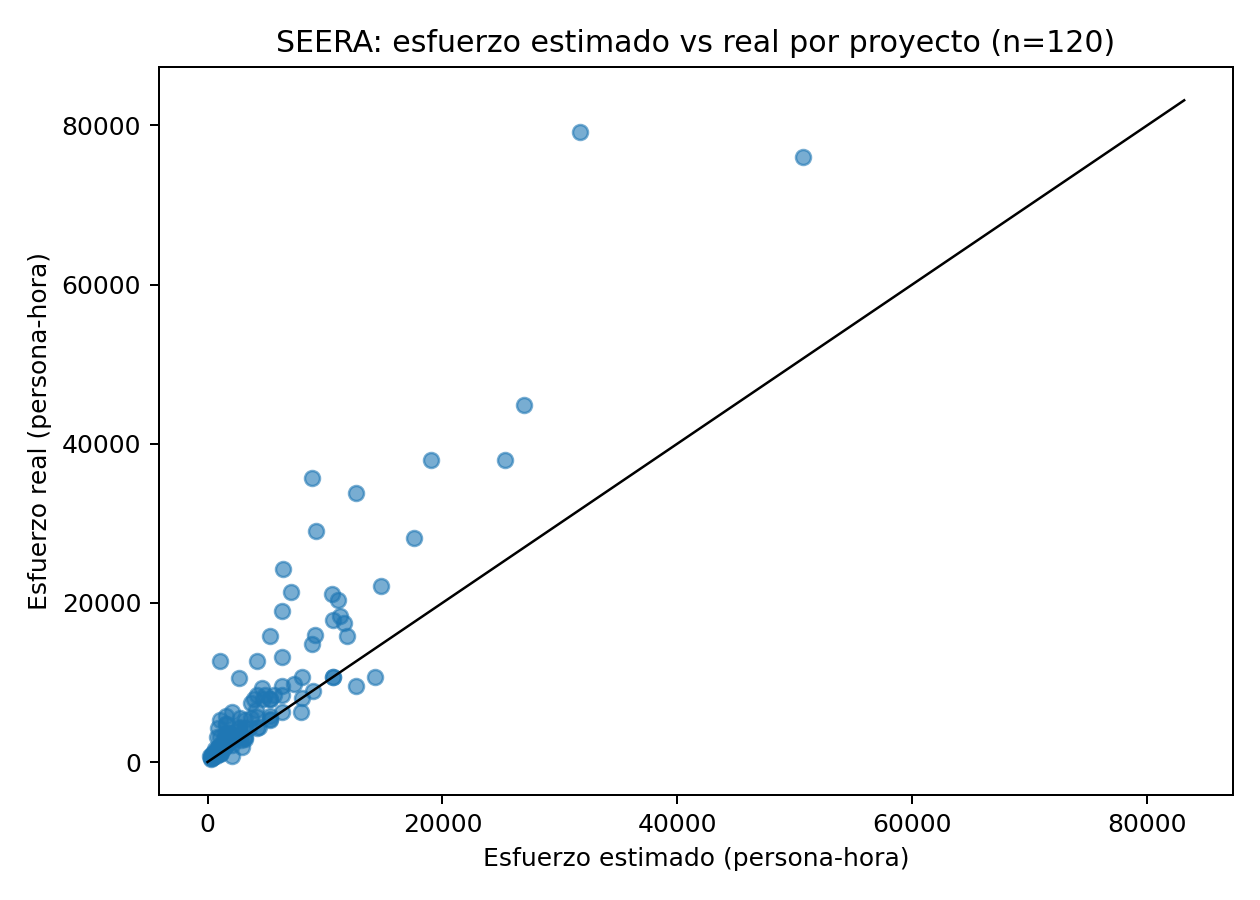
\includegraphics[width=0.95\linewidth]{../outputs/figures/seera_estimate_vs_actual.png}
\caption{Esfuerzo estimado contra esfuerzo real por proyecto en SEERA. Los puntos por encima de la diagonal corresponden a proyectos subestimados.}
\label{fig:seera}
\end{figure}

\begin{figure}[t]
\centering
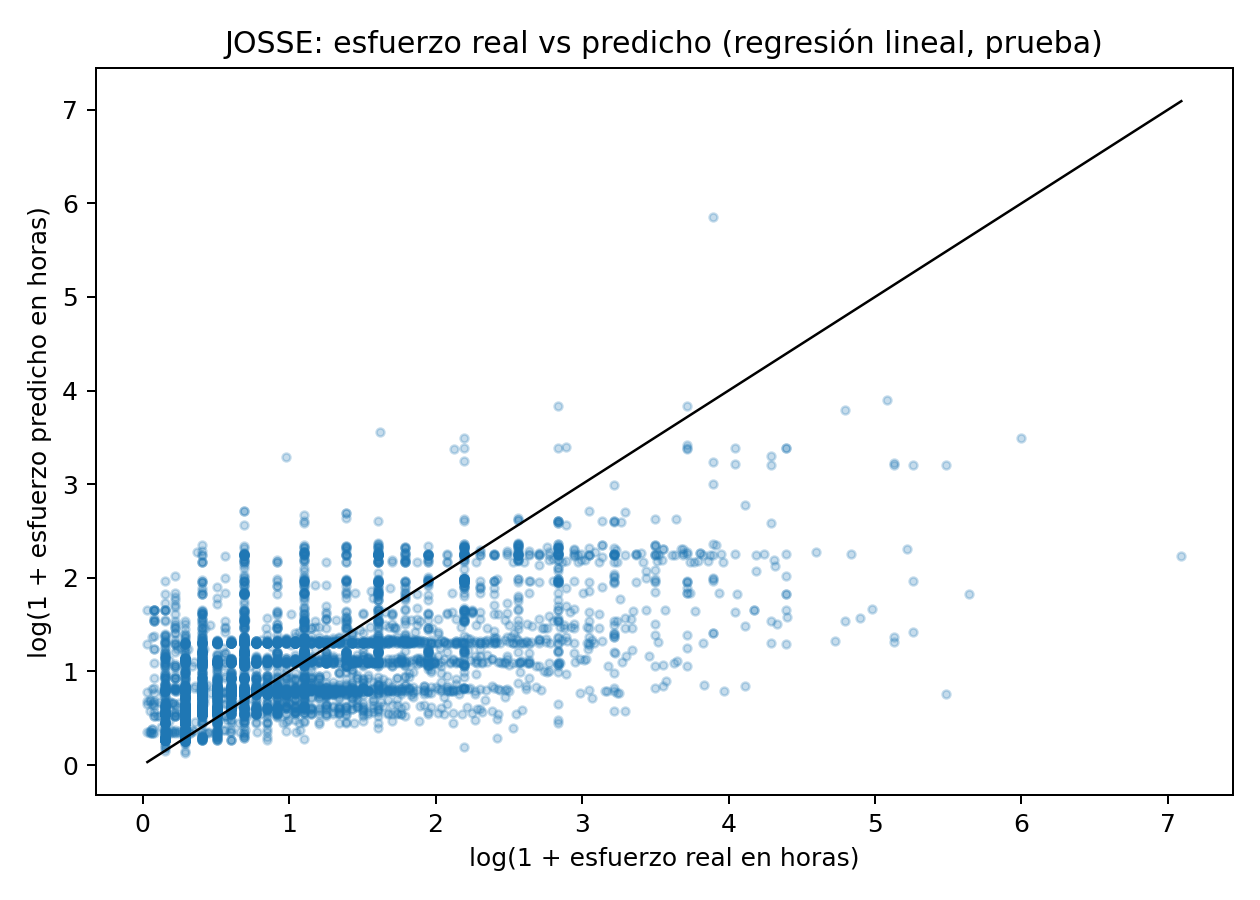
\includegraphics[width=0.95\linewidth]{../outputs/figures/actual_vs_predicted_josse.png}
\caption{Esfuerzo real contra esfuerzo predicho por la regresi\'on lineal en el conjunto de prueba de JOSSE.}
\label{fig:pred}
\end{figure}

\begin{figure}[t]
\centering
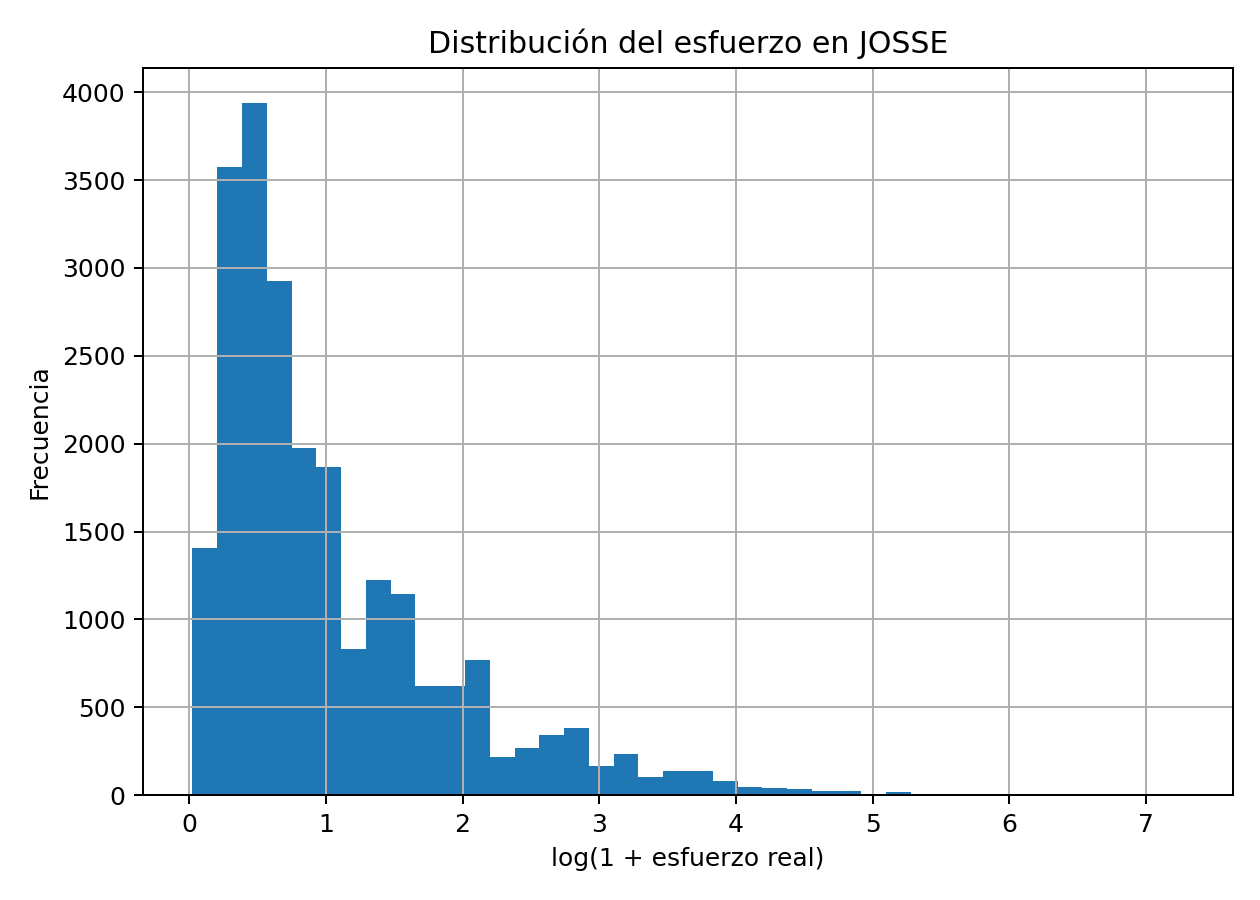
\includegraphics[width=0.95\linewidth]{../outputs/figures/effort_distribution_josse.png}
\caption{Distribuci\'on del esfuerzo real en JOSSE (escala logar\'itmica).}
\label{fig:distjosse}
\end{figure}

\begin{figure}[t]
\centering
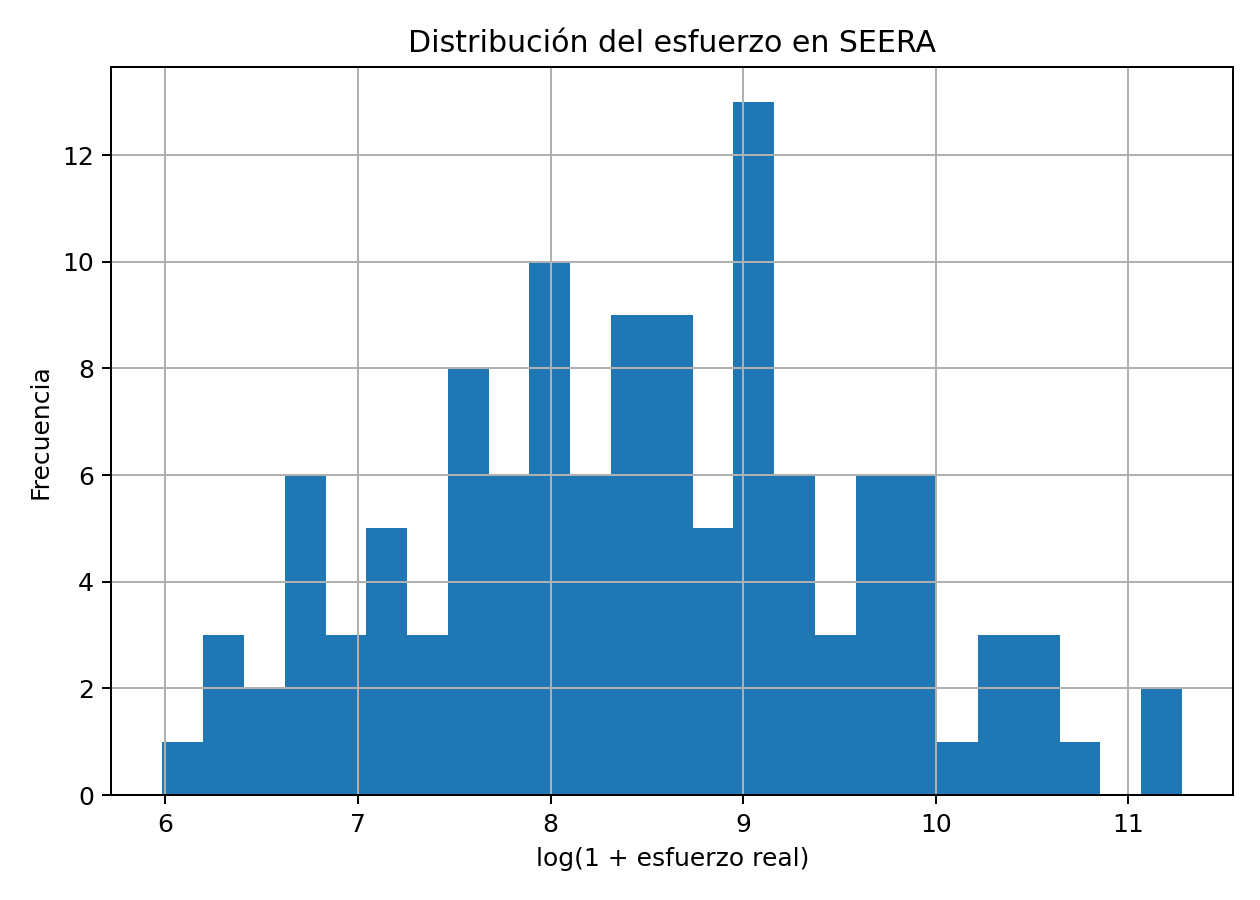
\includegraphics[width=0.95\linewidth]{../outputs/figures/effort_distribution_seera.png}
\caption{Distribuci\'on del esfuerzo real en SEERA (escala logar\'itmica).}
\label{fig:distseera}
\end{figure}

\begin{figure}[t]
\centering
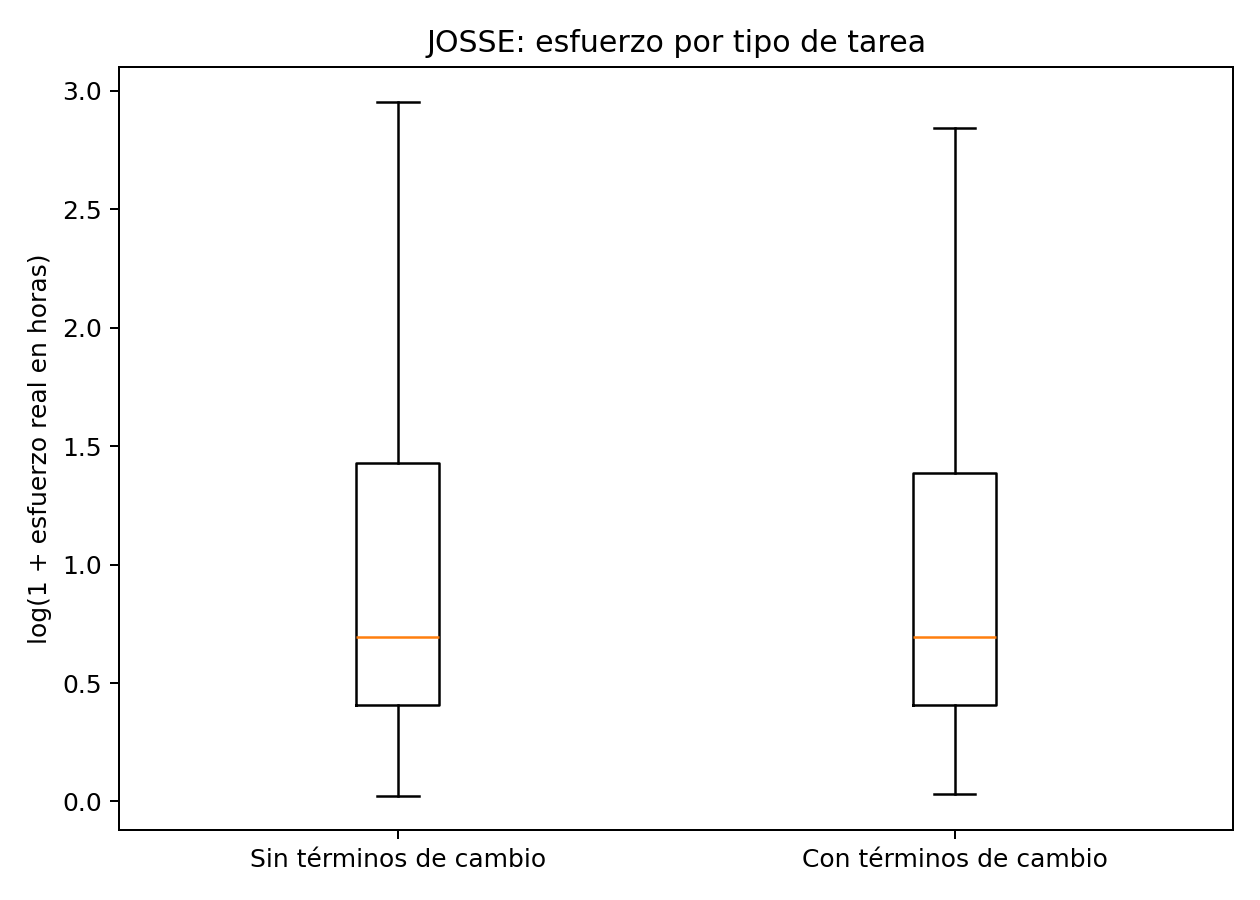
\includegraphics[width=0.95\linewidth]{../outputs/figures/josse_change_boxplot.png}
\caption{Esfuerzo real por tipo de tarea en JOSSE (sin valores at\'ipicos).}
\label{fig:boxplot}
\end{figure}


\section{Discusión}
Los tres resultados convergen hacia las premisas del modelo de estimación integral propuesto para Fresnillo.

Primero, H1 queda apoyada en ambos datasets. El juicio experto ordena pero no dimensiona: en JOSSE seis de cada diez estimaciones expertas exceden el umbral de $\pm$15\,\%, y en SEERA, el dataset cuyo contexto de restricciones técnicas y económicas más se parece al de proveedores municipales mexicanos, ocho de cada diez proyectos costaron más esfuerzo del estimado, con una mediana de +\desvSeera. Para un ayuntamiento, este número tiene lectura directa: una cotización aceptada por intuición tiene alta probabilidad de derivar en sobrecostos, renegociaciones o proyectos abandonados. Para un proveedor, subestimar 59\,\% el esfuerzo puede significar operar varios meses por debajo del costo real.

Segundo, H3 también queda apoyada: las variables observables en etapas tempranas (el texto de la solicitud en JOSSE; las características del proyecto y de la organización en SEERA) superan de forma consistente a la línea base. El $R^2$ de \rdosSeeraRF{} en SEERA indica que una parte sustancial de la variación del esfuerzo es explicable con información disponible antes de ejecutar el proyecto. Esto no implica que un modelo entrenado en datos públicos sea transferible a Fresnillo; implica que capturar variables estructuradas desde el inicio tiene valor predictivo y que un instrumento local de captura es la inversión correcta.

Tercero, el resultado nulo de H2 delimita el diseño: detectar cambios mediante palabras clave en texto libre no funciona. Esto respalda la decisión del prototipo EMPS-Fresnillo de capturar los cambios de forma estructurada (tipo de cambio, fase del proyecto, artefactos afectados, claridad, riesgo y regla de cobro) en lugar de inferirlos del lenguaje natural. La consecuencia metodológica es directa: el costo de un cambio se calcula a partir de variables de impacto y se presenta como rango justificado, no como cifra manual ni como inferencia léxica.

En conjunto, la evidencia pública justifica la siguiente fase de la investigación: el prototipo EMPS-Fresnillo como instrumento de captura local que registra proyectos, módulos, historias, equipo, cambios, parámetros fiscales y laborales mexicanos (IMSS, INFONAVIT, ISN, IVA, ISR), materiales, flujo de efectivo y resultados reales, para contrastar la hipótesis general con casos municipales documentados.

\section{Amenazas a la validez}
\textbf{Validez externa.} JOSSE proviene de proyectos de código abierto y SEERA de organizaciones de otro contexto nacional; ninguno representa directamente a Fresnillo. Los resultados se usan como evidencia de premisas, no como calibración local.
\textbf{Validez de constructo.} La variable de cambio en JOSSE se construyó con palabras clave, aproximación que el propio análisis mostró insuficiente; el esfuerzo real proviene de worklogs autorreportados, con el subregistro conocido de ese mecanismo.
\textbf{Validez interna.} En SEERA el tamaño muestral es reducido ($n=\nSeera$, 30 casos de prueba), por lo que el $R^2$ del bosque aleatorio debe leerse con cautela; se reporta junto a la regresión lineal y la línea base para transparentar el rango. En JOSSE, la inclusión de la estimación experta como subconjunto separado evita imputar masivamente valores faltantes.
\textbf{Reproducibilidad.} Todo el pipeline (descarga, preparación, análisis y generación de tablas y figuras) está automatizado en scripts y los resultados del texto se insertan de manera programática desde las tablas generadas, sin transcripción manual.

\section{Conclusiones y trabajo futuro}
Este avance aporta la fase cuantitativa preliminar de una metodología de estimación temprana integral para proyectos de software municipales. Con \nJosse{} tareas y \nSeera{} proyectos públicos se documentó que las estimaciones basadas en juicio fallan mayoritariamente el umbral de $\pm$15\,\% (H1), que la subestimación es sistemática en entornos restringidos (+\desvSeera{} de desviación mediana), que las variables tempranas estructuradas superan a la línea base (H3, $R^2$ de \rdosJosseLin{} a \rdosSeeraRF) y que la detección léxica de cambios es insuficiente (H2), lo que justifica la captura estructurada.

El trabajo futuro consiste en operar el prototipo EMPS-Fresnillo como instrumento de campo: capturar casos municipales con estimación y resultado real, medir la desviación con los mismos indicadores aquí utilizados (MdMRE, PRED(15)), contrastar los cinco modos de desarrollo considerados (tradicional, asistido, híbrido, codificación con prompts y bajo código) y recalibrar los factores del motor de estimación con evidencia local. La hipótesis general se considerará apoyada si la estimación integral identifica riesgos que una cotización tradicional no muestra: subestimación técnica, cambios no cotizados, insuficiencia de flujo de efectivo y mantenimiento omitido.

\bibliographystyle{apalike}
\bibliography{references}
\end{document}
